\textbf{Agenda}

Pada bab ini kita akan membahas beberapa topik yang berhubungan dengan tipe data dan Indentifier yaitu:

\minitoc

\section{Tipe Data dan Identifier}\label{tipe-data-dan-identifier}

\index{Program}Program adalah kumpulan instruksi yang disusun sedemikian rupa sehingga
mempunyai urutan nalar yang tepat untuk menyelesaikan suatu persoalan.
Instruksi-instruksi yang digunakan dalam pemrograman mengacu pada suatu
bahasa pemrograman tertentu, pada buku ini menggunakan bahasa
pemrograman C++, sehingga penulisan program pada buku ini mengikuti tata
bahasa C++.

Segala sesuatu yang diproses oleh program adalah data. Dalam hal ini
data adalah elemen-elemen yang digunakan untuk menjelaskan segala
sesuatu yang mempunyai besaran (ukuran/ nilai), seperti misalnya
\textbf{umur} besarannya bisa berupa biangan desimal \textbf{42.5}
(maksudnya 42\textonehalf{} tahun), \textbf{golongan} seorang karyawan besarannya
bisa berupa sebuah karakter A (maksudnya goongan A) dan sebagainya.
Bahasa C++ menyimpan besaran-besaran tersebut di memori utama untuk
dikelola oleh program, sehingga perlu dilakukan pengaturan pemakaian
memori, oleh karena itu dalam bahasa pemrograman selalu terdapat
istilah-istilah yang bernama \textbf{Tipe Data}, \textbf{Variabel} dan
\textbf{Konstanta}\index{konstanta}.

Identifier (pengenal) adalah suatu nama yang digunakan program untuk
merujuk ke suatu lokasi memori tertentu agar nilai pada lokasi tersebut
dapat diakses. Alamat lokasi memori sebenarnya berupa angka angka
heksadesimal\index{heksadesimal}, namun pada bahasa pemrograman
setingkat C++ (middle level programming language)
\index{middle level programming language} dan di atasnya, telah
mengubahnya dalam bentuk identifier (pengenal) yaitu berupa suatu huruf
atau kata (label) sehingga kita tidak perlu mengetahu alamat yang
sesungguhnya dan dengan identifier\index{identifier} (label) akan lebih mudah untuk
diingat.

\section{Tipe Data Bahasa C++}\label{tipe-data-bahasa-c}

Data yang dapat dikelola oleh program bisa bermacam-macam, seperti
misalnya bilangan bulat (\emph{integer}), bilangan dengan desimal
(\emph{floating point}), huruf (\emph{character}), dan sebagainya. Oleh
sebab itu ketika kita akan memakai suatu lokasi memori tertentu untuk
menyimpan nilai diperlukan 2 hal, yaitu \texttt{identifier} sebagai
pengenal (label) lokasi memori yang digunakan dan \texttt{tipe\ data},
yaitu besaran yang menentukan ukuran memori yang dialokasikan. Sekali
suatu identifier sudah dialokasikan dengan tipe data tertentu besarnya
ruang yang digunakan tidak bisa diubah. Bahasa C++ mengenal tipe-tipe
tabel berikut ini.


\begin{longtable}[]{@{}lll@{}}
\toprule
Tipe Data & Ukuran & Jangkauan Nilai Yang dapat Ditampung\tabularnewline
\midrule
\endhead
bool & 1 byte & True or false\tabularnewline
unsigned short int & 2 bytes & 0 to 65,535\tabularnewline
short int & 2 bytes & --32,768 to 32,767\tabularnewline
unsigned long int & 4 bytes & 0 to 4,294,967,295\tabularnewline
long int & 4 bytes & --2,147,483,648 to 2,147,483,647\tabularnewline
int (16 bit) & 2 bytes & --32,768 to 32,767\tabularnewline
int (32 bit) & 4 bytes & --2,147,483,648 to 2,147,483,647\tabularnewline
unsigned int (16 bit) & 2 bytes & 0 to 65,535\tabularnewline
unsigned int (32 bit) & 4 bytes & 0 to 4,294,967,295\tabularnewline
char & 1 byte & 256 character values\tabularnewline
float & 4 bytes & 1.2e--38 to 3.4e38\tabularnewline
double & 8 bytes & 2.2e--308 to 1.8e308\tabularnewline
\bottomrule

\end{longtable}


\section{Variabel dan Konstanta}\label{variabel-dan-konstanta}

Nilai yang tersimpan di memori dan dikenal melalui identifier tersebut
terdiri dari variabel dan konstanta. Perbedaan diantara keduanya adalah
bahwa variabel (sesuai dengan namanya) nilainya dapat diubah-ubah pada
saat program dieksekusi, sedangkan konstanta nilainya tidak dapat diubah
(\texttt{konstan\ =\ tetap}).

Sebelum suatu variabel atau konstanta dapat digunakan, tempat pada
memori harus dipesan terlebih dahulu, mekanisme ini dinamalan deklarasi.
Deklarasi dilakukan dengan cara menuliskan tipe data (ukuran memori yang
dibutuhkan) dan diikuti dengan nama pengenal (nama variabel), jika
dikehendaki bisa juga suatu variabel langsung diinisialisasi dengan
suatu nilai. Pengenal (identifier) bisa terdiri dari sebuah huruf atau
kombinasi antara huruf dengan angka dengan syarat.

\begin{itemize}

\item
  Harus diawali dengan huruf
\item
  Tidak boleh memakai karakter khusus kecuali \$ dan garis bawah (\_)
\item
  Tidak boleh sama dengan kata kunci yang digunakan pada C++
\item
  Bersifat case sensitif (huruf besar dan kecil dibedakan)
\end{itemize}

Walaupun demikian, sebaiknya memberikan nama pengenal variabel sesuai
dengan isi dari variabel tersebut, sebab walaupun nama variabel
``\textbf{c21i8k}'' untuk menyimpan nama mahasiswa adalah valid
(diperbolehkan), namun akan lebih mudah dimengerti jika identifier yang
dipilih adalah ``\textbf{nama}''.

Konstanta mirip dengan variabel, hanya saja nilainya konstan, tidak
dapat diubah-ubah. Untuk dapat membuat konstanta diperlukan inisialisasi
ketika konstanta dibuat dan setelah itu nilainya tidak dapat diubah. C++
mempunyai 2 macam konstanta, yaitu konstanta literal dan konstanta
simbolik. Berikut ini adalah contoh deklarasi variabel:

\begin{lstlisting}[language=c++, numbers=none]
int harga;
\end{lstlisting}

Yang dimaksud dengan konstanta literal adalah suatu nilai yang ditulis
pada kode program. Sebagai contoh misalnya :

\begin{lstlisting}[language=c++, numbers=none]
int usiaku = 42;
\end{lstlisting}

Nilai 42 tidak dapat menerima nilai lain dan nilai tersebut bersifat
tetap. Perhatikan dalam hal ini identifier ``usiaku'' adalah variabel
(bukan konstanta), yang dinamakan konstanta literal adalah nilai ``42''
tersebut.

Konstanta simbolik adalah konstanta yang direpresentasikan dengan suatu
nama, sama seperti variabel, namun berbeda dengan variabel setelah suatu
konstanta diinisialisasi dengan suatu nilai maka nilainya tidak dapat
diubah. Ada 2 cara untuk mendeklarasikan konstanta simbolik, yaitu
dengan menggunakan preprocessor directive \texttt{\#define} dan yang
kedua adalah dengan memakai kata kunci \texttt{const}. Berikut ini
contoh mendeklarasikan dan menginisialisasi konstanta :

\begin{lstlisting}[language=c++, numbers=none]
#define kapasitas 15
\end{lstlisting}

Perhatikan bahwa \texttt{kapasitas} tidak mempunyai tipe data tertentu
(int, char dsb.). Preprosessor akan melakukan substitusi berupa teks,
setiap ada akses terhadap kata \texttt{kapasitas}, akan digantikan
dengan teks 15. Karena preprosesor bekerja sebelum kompiler, kompiler
tidak mengenal konstanta \texttt{kapasitas}, yang dikenal hanyalah
bilangan 15.

\begin{quotation}
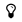
\includegraphics{../manuscript/images/tips}\textbf{TIPS} 

Walaupun
dengan memakai preprocessor directive \texttt{\#define} tampak mudah,
namun sebaiknya cara ini tidak digunakan, karena sudah dinyatakan usang
pada standard C++ .
\end{quotation}
 

Cara yang kedua untuk menginisialisasi sebuah konstanta adalah dengan
memakai kata kunci const seperti berikut :

\begin{lstlisting}[language=c++, numbers=none]
const int usiaku = 42;
\end{lstlisting}

Contoh diatas adalah mendeklarasikan konstanta simbolik bernama usiaku
bertipe int dan diinisialisasi dengan nilai 42. Setelah baris ini simbol
(identifier) bernama usiaku tidak dapat diubah-ubah nilainya. Keuntungan
pembuatan konstanta dengan cara ini adalah lebih mudah dipelihara dan
mencegah adanya kesalahan dan yang paling penting adalah bahwa konstanta
ini mempunyai tipe data dan kompiler dapat mengharuskan konstanta ini
diperlakukan sebagai tipe data tersebut.

\subsubsection*{Contoh Tipe data dan Identifier.}

\begin{enumerate}

\item
  Buka Qt Creator dan buat project Qt Console Application baru dengan
  nama contoh \ref{contoh2-1}, kemudian tulis kode berikut.

\lstinputlisting[language=c++, caption=Tipe data dan Identifier, label=contoh2-1]{../code/contoh2-1.cpp}

\item
  Kemudian jalankan kode diatas dengan menekan tombol Ctrl+R, outputnya
  adalah sebagai berikut.

\begin{lcverbatim}
Panjang =15
lebar =12
\end{lcverbatim}

\end{enumerate}


\subsubsection*{Keterangan}

\begin{itemize}

\item
  Pada program di atas variabel panjang dan lebar dideklarasikan bertipe
  int.
\item
  Kemudian variabel panjang diberi nilai 15 (integer) dan lebar diberi
  nilai 12 (integer), tampak bahwa nilai dari variabel tersebut dapat
  diubah.
\item
  Pada baris berikutnya nilai dari variabel dapat diakses untuk dicetak
  ke layar.
\end{itemize}

\section{Statement}\label{statement}

Dalam bahasa C++, sebuah statement mengontrol urutan pengerjaan
eksekusi, mengevaluasi ekspresi atau tidak mengejakan apapun (\emph{null
statement}). Semua statement C++ diakhiri dengan titik koma (;), sebagai
contoh misalnya :

\begin{lstlisting}[language=c++, numbers=none]
x = a + b;
\end{lstlisting}

Pernyataan tersebut bukanlah suatu pernyataan persamaan aljabar dalam
matematika yang artinya x sama dengan a + b, melainkan memberi nilai x
dengan hasil penjumlahan a dengan b. Pada statement ini terjadi 2 urutan
pengerjaan, yaitu pertama menambahkan a dengan b, kemudian yang kedua
memberikan hasil perhitungan tersebut ke variabel x dengan operator
pengerjaan (=). Walaupun pada pernyataan tersebut terdapat 2 pekerjaan,
namun merupakan sebuah statement dan oleh karena itu diakhiri hanya
dengan sebuah titik koma (;) saja. Hasil penjumlahan a dengan b ini
disebut ekspresi, sedangkan sama dengan (=) dan plus (+) dinamakan
operator yang akan dibahas berikut ini.

\begin{quotation}
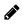
\includegraphics{../manuscript/images/pencil} \textbf{CATATAN}
 
 Operator pengerjaan = akan mengambil nilai apapun yang ada disebelah
 kanannya kenudian memberikannya kepada apapun yang berada di sebelah
 kirinya. C++ mengenal juga operator pembanding == yang mempunyai
 arti berbeda dengan operator sama dengan =, akan dibahas lebih
 detail pada sub bab berikut ini.
\end{quotation}


\section{Operator dan Ekspresi}\label{operator-dan-ekspresi}

Operator adalah suatu simbol yang digunakan untuk melakukan suatu
operasi. Operator mempunyai beberapa kategori, antara lain : Aritmatika,
Pengerjaan, Hubungan dan Logika. Operator Aritmatika adalah operator
yang digunakan untuk melakukan operasi aritmatika seperti misalnya
penjumlahan, pengurangan, perkalian dan pembagian. Simbol untuk operator
aritmatika ini adalah : +, -, *, / dan \%. Berikut ini adalah
operator-operator yang dikenal pada bahasa pemrograman C++.

\begin{longtable}[]{@{}llll@{}}
\toprule
\begin{minipage}[b]{0.52\columnwidth}\raggedright\strut
Kategori
\strut\end{minipage} &
\begin{minipage}[b]{0.17\columnwidth}\raggedright\strut
Operator
\strut\end{minipage} &
\begin{minipage}[b]{0.14\columnwidth}\raggedright\strut
Arah Proses
\strut\end{minipage} &
\begin{minipage}[b]{0.05\columnwidth}\raggedright\strut
Jenjang
\strut\end{minipage}\tabularnewline
\midrule
\endhead
\begin{minipage}[t]{0.52\columnwidth}\raggedright\strut
Kurung, indeks larik dan elemen struktur data
\strut\end{minipage} &
\begin{minipage}[t]{0.17\columnwidth}\raggedright\strut
() {[}{]} . -\textgreater{}
\strut\end{minipage} &
\begin{minipage}[t]{0.14\columnwidth}\raggedright\strut
Kiri - Kanan
\strut\end{minipage} &
\begin{minipage}[t]{0.05\columnwidth}\raggedright\strut
1
\strut\end{minipage}\tabularnewline
\begin{minipage}[t]{0.52\columnwidth}\raggedright\strut
Operator Unary
\strut\end{minipage} &
\begin{minipage}[t]{0.17\columnwidth}\raggedright\strut
! \textasciitilde{} - ++ --
\strut\end{minipage} &
\begin{minipage}[t]{0.14\columnwidth}\raggedright\strut
Kanan -- Kiri
\strut\end{minipage} &
\begin{minipage}[t]{0.05\columnwidth}\raggedright\strut
2
\strut\end{minipage}\tabularnewline
\begin{minipage}[t]{0.52\columnwidth}\raggedright\strut
Operator Aritmatika Perkalian, Pembagian dan Sisa Pembagian
\strut\end{minipage} &
\begin{minipage}[t]{0.17\columnwidth}\raggedright\strut
* / \%
\strut\end{minipage} &
\begin{minipage}[t]{0.14\columnwidth}\raggedright\strut
Kiri -- Kanan
\strut\end{minipage} &
\begin{minipage}[t]{0.05\columnwidth}\raggedright\strut
3
\strut\end{minipage}\tabularnewline
\begin{minipage}[t]{0.52\columnwidth}\raggedright\strut
Operator aritmatika Pertambahan dan Pengurangan
\strut\end{minipage} &
\begin{minipage}[t]{0.17\columnwidth}\raggedright\strut
+ -
\strut\end{minipage} &
\begin{minipage}[t]{0.14\columnwidth}\raggedright\strut
Kiri -- Kanan
\strut\end{minipage} &
\begin{minipage}[t]{0.05\columnwidth}\raggedright\strut
4
\strut\end{minipage}\tabularnewline
\begin{minipage}[t]{0.52\columnwidth}\raggedright\strut
Operator Bitwise Pergeseran Bit
\strut\end{minipage} &
\begin{minipage}[t]{0.17\columnwidth}\raggedright\strut
\textless{}\textless{} \textgreater{}\textgreater{}
\strut\end{minipage} &
\begin{minipage}[t]{0.14\columnwidth}\raggedright\strut
Kiri -- Kanan
\strut\end{minipage} &
\begin{minipage}[t]{0.05\columnwidth}\raggedright\strut
5
\strut\end{minipage}\tabularnewline
\begin{minipage}[t]{0.52\columnwidth}\raggedright\strut
Operator Hubungan
\strut\end{minipage} &
\begin{minipage}[t]{0.17\columnwidth}\raggedright\strut
\textless{} \textless{}= \textgreater{} \textgreater{}=
\strut\end{minipage} &
\begin{minipage}[t]{0.14\columnwidth}\raggedright\strut
Kiri -- Kanan
\strut\end{minipage} &
\begin{minipage}[t]{0.05\columnwidth}\raggedright\strut
6
\strut\end{minipage}\tabularnewline
\begin{minipage}[t]{0.52\columnwidth}\raggedright\strut
Operator Hubungan Kesamaan dan Ketidaksamaan
\strut\end{minipage} &
\begin{minipage}[t]{0.17\columnwidth}\raggedright\strut
== !=
\strut\end{minipage} &
\begin{minipage}[t]{0.14\columnwidth}\raggedright\strut
Kiri -- Kanan
\strut\end{minipage} &
\begin{minipage}[t]{0.05\columnwidth}\raggedright\strut
7
\strut\end{minipage}\tabularnewline
\begin{minipage}[t]{0.52\columnwidth}\raggedright\strut
Operator Bitwise AND
\strut\end{minipage} &
\begin{minipage}[t]{0.17\columnwidth}\raggedright\strut
\&
\strut\end{minipage} &
\begin{minipage}[t]{0.14\columnwidth}\raggedright\strut
Kiri -- Kanan
\strut\end{minipage} &
\begin{minipage}[t]{0.05\columnwidth}\raggedright\strut
8
\strut\end{minipage}\tabularnewline
\begin{minipage}[t]{0.52\columnwidth}\raggedright\strut
Operator Bitwise XOR
\strut\end{minipage} &
\begin{minipage}[t]{0.17\columnwidth}\raggedright\strut
\^{}
\strut\end{minipage} &
\begin{minipage}[t]{0.14\columnwidth}\raggedright\strut
Kiri -- Kanan
\strut\end{minipage} &
\begin{minipage}[t]{0.05\columnwidth}\raggedright\strut
9
\strut\end{minipage}\tabularnewline
\begin{minipage}[t]{0.52\columnwidth}\raggedright\strut
Operator Bitwise OR
\strut\end{minipage} &
\begin{minipage}[t]{0.17\columnwidth}\raggedright\strut
\texttt{\textbar{}}
\strut\end{minipage} &
\begin{minipage}[t]{0.14\columnwidth}\raggedright\strut
Kiri -- Kanan
\strut\end{minipage} &
\begin{minipage}[t]{0.05\columnwidth}\raggedright\strut
10
\strut\end{minipage}\tabularnewline
\begin{minipage}[t]{0.52\columnwidth}\raggedright\strut
Operator Kondisi AND
\strut\end{minipage} &
\begin{minipage}[t]{0.17\columnwidth}\raggedright\strut
\&\&
\strut\end{minipage} &
\begin{minipage}[t]{0.14\columnwidth}\raggedright\strut
Kiri -- Kanan
\strut\end{minipage} &
\begin{minipage}[t]{0.05\columnwidth}\raggedright\strut
11
\strut\end{minipage}\tabularnewline
\begin{minipage}[t]{0.52\columnwidth}\raggedright\strut
Operator Kondisi OR
\strut\end{minipage} &
\begin{minipage}[t]{0.17\columnwidth}\raggedright\strut
\texttt{\textbar{}\textbar{}}
\strut\end{minipage} &
\begin{minipage}[t]{0.14\columnwidth}\raggedright\strut
Kiri -- Kanan
\strut\end{minipage} &
\begin{minipage}[t]{0.05\columnwidth}\raggedright\strut
12
\strut\end{minipage}\tabularnewline
\begin{minipage}[t]{0.52\columnwidth}\raggedright\strut
Operator Ternary ?
\strut\end{minipage} &
\begin{minipage}[t]{0.17\columnwidth}\raggedright\strut
\texttt{\textbar{}}
\strut\end{minipage} &
\begin{minipage}[t]{0.14\columnwidth}\raggedright\strut
Kanan -- Kiri
\strut\end{minipage} &
\begin{minipage}[t]{0.05\columnwidth}\raggedright\strut
13
\strut\end{minipage}\tabularnewline
\begin{minipage}[t]{0.52\columnwidth}\raggedright\strut
Operator Pengerjaan Aritmatika
\strut\end{minipage} &
\begin{minipage}[t]{0.17\columnwidth}\raggedright\strut
= += -= *= /= \%=
\strut\end{minipage} &
\begin{minipage}[t]{0.14\columnwidth}\raggedright\strut
Kanan -- Kiri
\strut\end{minipage} &
\begin{minipage}[t]{0.05\columnwidth}\raggedright\strut
14
\strut\end{minipage}\tabularnewline
\begin{minipage}[t]{0.52\columnwidth}\raggedright\strut
Operator Pengerjaan Bitwise
\strut\end{minipage} &
\begin{minipage}[t]{0.17\columnwidth}\raggedright\strut
\texttt{\&=\ \^{}=\ \textbar{}=\ \textless{}\textless{}=\ \textgreater{}\textgreater{}=}
\strut\end{minipage} &
\begin{minipage}[t]{0.14\columnwidth}\raggedright\strut
Kanan -- Kiri
\strut\end{minipage} &
\begin{minipage}[t]{0.05\columnwidth}\raggedright\strut
15
\strut\end{minipage}\tabularnewline
\begin{minipage}[t]{0.52\columnwidth}\raggedright\strut
Operator Koma
\strut\end{minipage} &
\begin{minipage}[t]{0.17\columnwidth}\raggedright\strut
,
\strut\end{minipage} &
\begin{minipage}[t]{0.14\columnwidth}\raggedright\strut
Kiri -- Kanan
\strut\end{minipage} &
\begin{minipage}[t]{0.05\columnwidth}\raggedright\strut
16
\strut\end{minipage}\tabularnewline
\bottomrule
\end{longtable}

Ekspresi adalah suatu peryataan yang menghasilkan suatu nilai, bisa
berasal dari sebuah variabel maupun kumpulan variabel-variabel yang
dioperasikan dengan suatu operator, jadi hasil akhir dari suatu ekspresi
adalah suatu nilai yang mempunyai besaran dan tipe data tertentu.

Pernyataan berikut ini yang disebut ekspresi adalah 15, 12 dan ``panjang
* lebar'' yang menghasilkan nilai 15, 12 dan 180:

\begin{lstlisting}[language=c++, numbers=none]
panjang = 15;
lebar = 12;
luas = panjang * lebar ;
\end{lstlisting}

\textbf{Keterangan :}

\begin{itemize}

\item
  Pada baris pertama dan kedua di atas digunakan hanya sebuah operator
  \texttt{=} (yaitu jenjang ke 14), arah proses dari kanan ke kiri,
  sehingga yang dilakukan :
\item
  Ekspresi : \texttt{15}, diberikan kepada variabel \texttt{panjang}
  (dibaca dari kanan ke kiri).
\item
  Ekspresi : \texttt{12}, diberikan kepada variabel \texttt{lebar}
  (dibaca dari kanan ke kiri).
\item
  Pada baris ketiga terdapat 2 operator, yaitu operator =  (jenjang
  ke 14) dan \texttt{*} operator = (yaitu jenjang ke 3).
  Jenjang menunjukkan operator yang akan dikerjakan terlebih dahulu,
  jika dalam sebuah ungkapan terdapat lebih dari satu jenis operator.
  Jenjang nomor 1 adalah jenjang yang paling tinggi, maka pada
  pernyataan di atas yang akan dikerjakan terlebih dahulu adalah orator
  \texttt{*} baru kemudian operator =, sehingga yang dilakukan:
  - Ekspresi : \texttt{panjang\ *\ lebar} , berarti \texttt{panjang}
  dikalikan \texttt{lebar} (dibaca dari kiri ke kanan), menghasilkan
  nilai integer \texttt{180}. - Berikutnya operator = mengoperasikan
  hasil ekspresi tersebut, yaitu nilai integer \texttt{180} diberikan
  kepada variabel \texttt{luas} (dibaca dari kanan ke kiri).
\end{itemize}

\begin{quotation}
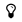
\includegraphics{../manuscript/images/tips}\textbf{TIPS}

Operator
( dan ) dapat dipakai untuk merubah jenjang suatu ekspresi
menjadi jenjang tertinggi, sehingga akan diproses terlebih dahulu.
\end{quotation}


\subsection{ Operator Unary}\label{a-operator-unary}

Operator unary adalah operator yang hanya menggunakan sebuah operand
saja, operator unary yang dipakai pada kebanyakan bahasa pemrograman
adalah operator unary minus (-). Operator unary ditulis sebelum operand,
operator unary ``-'' berbeda dengan operator aritmatika ``-'' yang
membutuhkan dua operand. Dalam bahasa C++ disediakan bermacam-macam
operator unary.

\begin{longtable}[]{@{}ll@{}}
\toprule
Operator & Arti\tabularnewline
\midrule
\endhead
- & Unary minus\tabularnewline
++ & Peningkatan dengan nilai penambahan 1\tabularnewline
-- & Penurunan dengan nilai pengurangan 1\tabularnewline
! & Unary not\tabularnewline
\textasciitilde{} & Operator unary komplemen satu (bitwise
NOT)\tabularnewline
\bottomrule
\end{longtable}

\subsection{Operator Unary Minus}\label{b-operator-unary-minus}

Operator ini dipakai untuk memberi nilai minus suatu nilai numerik
(bukan pengurangan). Misalnya ungkapan : \texttt{A\ +\ -\ B\ *\ C} akan
diartikan \texttt{A\ +\ (-B)\ *\ C}. Operator unary ``-'' ditulis di
depan operand.

\subsection{Operator Unary ++ dan --}\label{c-operator-unary-dan}

Operator unary ``++'' dan ``--'' merupakan operator khusus yang ada di
bahasa C. Operator ``++'' akan menambahkan nilai 1 ke pengenal yang
menggunakannya sedangkan operator ``--'' akan mengurangi dengan nilai
numerik 1. Operator unary tersebut jika dituliskan sebelum operand
disebut \emph{pre increment} sedangkan jika ditulis setelah operand
disebut \emph{post increment}. Perhatikan perbedaannya pada contoh
dibawah ini :

\begin{longtable}[]{@{}ll@{}}
\toprule
Post Increment & Pre Increment\tabularnewline
\midrule
\endhead
x = 5; & x = 5;\tabularnewline
a = x++; & a = ++x;\tabularnewline
------------------- & ----------------\tabularnewline
\textbf{Hasil:} & \textbf{Hasil:}\tabularnewline
x = 6 dan a = 5 & x = 6 dan a = 6\tabularnewline
\bottomrule
\end{longtable}

\subsection{Operator Pengerjaan}\label{d-operator-pengerjaan}

Operator pengerjaan atau disebut assignment operator, digunakan untuk
menempatkan nilai dari suatu ekspresi ke suatu pengenal. Operator yang
umum dipakai pada bahasa pemrograman adalah operator pengerjaan ``=''.
Selain operator pengerjaan ``='', bahasa C++ menyediakan beberapa
operator pengerjaan yang lain seperti tabel di bawah ini.

\begin{longtable}[]{@{}lll@{}}
\toprule
Operator & Contoh & Maksud/ Ekuivalen dengan\tabularnewline
\midrule
\endhead
= & a = b + c & Mengerjakan b+c ke a\tabularnewline
+= & a += 1 & a = a + 1\tabularnewline
-= & a -= b & a = a -- b\tabularnewline
*= & a *= b & a = a * b\tabularnewline
/= & a /= b & a = a / b\tabularnewline
\%= & a \%= b & a = a \% b\tabularnewline
\bottomrule
\end{longtable}

Tabel berikut ini memberikan contoh pemakaian operator-operator di atas,
misalnya variabel a dan b bernilai 10.

\begin{longtable}[]{@{}lll@{}}
\toprule
Statement & Ekuivalen dengan & Hasil Ungkapan\tabularnewline
\midrule
\endhead
a += 3 & a = a + 3 & a = 10 + 3 = 13\tabularnewline
a -= 2 & a = a - 2 & a = 10 -- 2 = 8\tabularnewline
a *= b/2 & a = a * (b/2) & a = 10 * (10/2) = 50\tabularnewline
a /= b -- 8 & a = a / (j -- 8) & a = 10 / (10-8) = 5\tabularnewline
\bottomrule
\end{longtable}

Dari contoh di atas terlihat bahwa operator pengerjaan mempunyai jenjang
yang lebih rendah dibanding operator aritmatika, sehingga operator
aritmatika dikerjakan terlebih dahulu.

C++ mengijinkan operator pengerjaan ditulis lebih dari satu kali pada
sebuah statement, misalnya :

\begin{lstlisting}[language=c++, numbers=none]
x = y = a * b;
\end{lstlisting}

Dalam hal ini yang dikerjakan adalah a dikalikan b terlebih dahulu
meudian hasilnya diberikan kepada variabel y dan hasil ekspresi y = a *
b diberikan kepada variabel x. sehingga misalnya a bernilai 8 dan b
bernilai 7, maka baik variabel x maupun y keduanya bernilai 15.

\subsection{Operator Hubungan}\label{e-operator-hubungan}

Operator hubungan (\emph{relational operator}) digunakan untuk
menunjukkan hubungan antara dua buah operand, hasil dari operator ini
adalah True atau False.

\begin{longtable}[]{@{}lll@{}}
\toprule
Operator & Jenjang & Arti\tabularnewline
\midrule
\endhead
\textless{} & 6 & Lebih kecil dari\tabularnewline
\textless{}= & 6 & Lebih kecil atau sama dengan\tabularnewline
\textgreater{} & 6 & Lebih besar dari\tabularnewline
\textgreater{}= & 6 & Lebih besar atau sama dengan\tabularnewline
== & 7 & Sama dengan\tabularnewline
!= & 7 & Tidak sama dengan\tabularnewline
\bottomrule
\end{longtable}

Berikut ini contoh hasil ekspresi jika a bernilai 5, b bernilai 7 dan c
bernilai `a'

\begin{longtable}[]{@{}lll@{}}
\toprule
Ungkapan Hubungan & Hasil & Nilai\tabularnewline
\midrule
\endhead
a == 5 & Benar & 1\tabularnewline
a == b & Salah & 0\tabularnewline
b \textless{} 7 & Salah & 0\tabularnewline
a \textless{}= 7 & Benar & 1\tabularnewline
(a+b) != 35 & Benar & 1\tabularnewline
c != `A' & Benar & 1\tabularnewline
c \textless{}= `z' & Benar & 1\tabularnewline
\bottomrule
\end{longtable}

\subsection{Operator Logika}\label{f-operator-logika}

Jika operator hubungan membandingkan hubungan antara dua buah operand,
maka operator logika (\emph{logical operator}) digunakan untuk
menggabungkan logika hasil dari operator-operator hubungan. Operator
logika menggabungkan \textbf{dua buah} nilai logika. Nilai logika adalah
nilai benar (True) atau salah (False).

\begin{longtable}[]{@{}lll@{}}
\toprule
Operator & Jenjang & Arti\tabularnewline
\midrule
\endhead
\&\& & 11 & Logika DAN (AND)\tabularnewline
\texttt{\textbar{}\textbar{}} & 12 & Logika ATAU (OR)\tabularnewline
\bottomrule
\end{longtable}

Selain dua operator logika ini, operator unary \textquotedblleft ! \textquotedblright (logika NOT) dapat digunakan untuk operasi logika.

\begin{longtable}[]{@{}lllll@{}}
\toprule
x & y & x \&\& y & x \texttt{\textbar{}\textbar{}} y & !x\tabularnewline
\midrule
\endhead
TRUE & TRUE & TRUE & TRUE & FALSE\tabularnewline
TRUE & FALSE & FALSE & TRUE & FALSE\tabularnewline
FALSE & TRUE & FALSE & TRUE & TRUE\tabularnewline
FALSE & FALSE & FALSE & FALSE & TRUE\tabularnewline
\bottomrule
\end{longtable}

Contoh : Misalnya A bernilai 5, B bernilai 7 dan C bernilai \textquotedblleft a \textquotedblright maka ungkapan dibawah ini mempunyai hasil akhir benar (True).

\begin{lstlisting}[language=c++, numbers=none]
A < B || B == 7 && C > 'z'
\end{lstlisting}

Hasil akhir benar (True) dari ekspresi logika tersebut didapat dari
langkah-langkah sebagai berikut:

\begin{enumerate}


\item
  Jenjang operator hubungan lebih tinggi dibandingkan dengan operator
  logika, jadi operator hubungan dikerjakan terlebih dahulu.
\item
  Operator logika ``\&\&'' mempunyai jenjang lebih tinggi dari operator
  ``\textbar{}\textbar{}'', sehingga operator ``\&\&'' dikerjakan
  terlebih dahulu.
\item
  Bagian yang paling akhir dikerjakan adalah operator
  ``\textbar{}\textbar{}'', sehingga hasil akhir logika bernilai logika
  benar atau True.
\end{enumerate}


